%This is an Appendix
%%=========================================

\chapter{Appendix B}
.

%%=========================================
\section{Hypothesis}

\subsection{Hypothesis dependent on community membership}
\begin{enumerate}
    \item We expect residents to be aware
    \item We expect commuters to be aware
    \item We expect marine workers to be aware
    \item We expect non-marine workers to be unaware
    \item We expect water leisure users to be aware
    \item We expect land leisure users to be unaware
    \end{enumerate}
\paragraph{}

\subsection{Hypothesis dependent on local knowledge}
\begin{enumerate}
    \item We expect subjects with professional interest in SLEs to be aware
    \item We expect subjects with primary knowledge about places which are on reclaimed land to be aware
    \item We expect subjects with a length of knowledge greater than 20 years of the area to be aware
    \item We expect subjects with a length of knowledge less than 1 year of the area to be unaware
    \item We expect subjects with many information sources about the place to be aware
    \item We expect subjects who chose to respond in Norwegian to be aware
\end{enumerate}
\paragraph{}

\subsection{Hypothesis dependent on awareness of changing climate}
\begin{enumerate}
    \item We expect subjects with many information sources about climate change to be aware
    \item We expect subjects with the information source of formal education to be aware
    \item We expect subjects with the information source of peer reviewed published papers to be aware
    \item We expect subjects who are more concerned about climate change to be aware
    \item We expect subjects who predict they will be impacted by flooding from SLEs to be aware
\end{enumerate}

\section{Summary Statistics }
Find below table \ref{table:summary_stats} which details the summary statistics for the responses to the survey. Table \ref{table:variable to questions} contains the codified variable name and what questions they respond to.



\begin{center}
\begin{table}[H]
    \centering
    \begin{tabular}{|l|l|l|l|l|l|l|}
    \hline
        variable name & mean & Std Dev. & min & max & range & skew  \\ \hline
        long\_know & 3.24 & 1.60 & 0 & 6 & 6 & 0.23 \\ \hline
        com\_mem & 1.44 & 0.89 & 0 & 6 & 6 & 2.10  \\ \hline
        com\_marine\_worker & 0.00 & 0.00 & 0 & 0 & 0 & Na   \\ \hline
        com\_worker & 0.12 & 0.33 & 0 & 1 & 1 & 2.26  \\ \hline
        com\_resident & 0.46 & 0.50 & 0 & 1 & 1 & 0.17  \\ \hline
        com\_student & 0.25 & 0.44 & 0 & 1 & 1 & 1.11 \\ \hline
        com\_play\_land & 0.27 & 0.45 & 0 & 1 & 1 & 1.00   \\ \hline
        com\_play\_water & 0.11 & 0.32 & 0 & 1 & 1 & 2.45  \\ \hline
        com\_commuter & 0.10 & 0.31 & 0 & 1 & 1 & 2.56   \\ \hline
        com\_other & 0.12 & 0.32 & 0 & 1 & 1 & 2.35   \\ \hline
        interest\_level & 3.17 & 0.95 & 1 & 5 & 4 & -0.16 \\ \hline
        ss\_now & 0.39 & 0.49 & 0 & 1 & 1 & 0.44  \\ \hline
        ss\_future & 0.31 & 0.46 & 0 & 1 & 1 & 0.83 \\ \hline
        ss\_tide & 0.88 & 0.32 & 0 & 1 & 1 & -2.35 \\ \hline
        info\_place\_sum & 1.94 & 1.34 & 0 & 8 & 8 & 1.61 \\ \hline
        info\_climate\_sum & 3.50 & 1.72 & 0 & 8 & 8 & 0.24 \\ \hline
        worry\_climate & 4.03 & 1.15 & 1 & 5 & 4 & -1.17 \\ \hline
        flood\_impact & 2.50 & 0.89 & 1 & 4 & 3 & 0.04  \\ \hline
        slr\_past & 0.17 & 0.43 & 0 & 2 & 2 & 2.47  \\ \hline
        slr\_future & 2.33 & 0.69 & 0 & 3 & 3 & -1.26 \\ \hline
        ss\_event & 0.58 & 0.93 & 0 & 7 & 7 & 2.78  \\ \hline
        survey\_access & 2.55 & 1.84 & 0 & 6 & 6 & 0.79  \\ \hline
        language & 0.57 & 0.50 & 0 & 1 & 1 & -0.27  \\ \hline
        place\_brattøra & 0.20 & 0.40 & 0 & 1 & 1 & 1.52  \\ \hline
        place\_grillstad & 0.24 & 0.43 & 0 & 1 & 1 & 1.19 \\ \hline
        place\_nidelva & 0.37 & 0.49 & 0 & 1 & 1 & 0.52 \\ \hline
        place\_skansen & 0.19 & 0.39 & 0 & 1 & 1 & 1.57 \\ \hline
    \end{tabular}
    \caption{Summary Statistics}
\label{table:summary_stats}
\end{table}
\end{center}


\begin{center}
\begin{table}[H]
    \centering
    \begin{tabular}{|l|l|}
    \hline
        variable name  & question asked \\ \hline
        long\_know & How long have you known this area? \\ \hline
        com\_mem  & What communities in this area are you part of? \\ \hline
        com\_marine\_worker & "" \\ \hline
        com\_worker & "" \\ \hline
        com\_resident & "" \\ \hline
        com\_student & "" \\ \hline
        com\_play\_land & "" \\ \hline
        com\_play\_water &  "" \\ \hline
        com\_commuter &  "" \\ \hline
        com\_other &  "" \\ \hline
        interest\_level & What is your level of interest in sea level extremes? \\ \hline
        ss\_now  & Which image shows the current 20-year storm surge? \\ \hline
        ss\_future  & Which image shows the 20-year storm surge projected for 2090? \\ \hline
        ss\_tide  & Which image displays the current high tide? \\ \hline
        info\_place\_sum & Where do you get information about changes to this place? \\ \hline
        info\_climate\_sum &  "Where do you get information about changes to the climate" \\ \hline
        worry\_climate &  Are you concerned about climate change? \\ \hline
        flood\_impact &  How would flooding associated with sea level extremes in this area affect you? \\ \hline
        slr\_past & How much do you think the sea level has changed here in the past 30 years? \\ \hline
        slr\_future & How much do you think the sea level will change in the next 30 years? \\ \hline
        ss\_event & Please tick if you remember any of these dates when coastal  \\ \newline
        & sea levels in Trondheim were over 2m \\ \hline
        survey\_access  & How did you access this survey? \\ \hline
        language  & Determined from which survey subjects filled out \\ \hline
        place\_brattøra  & "" \\ \hline
        place\_grillstad  & "" \\ \hline
        place\_nidelva & "" \\ \hline
        place\_skansen & "" \\ \hline
    \end{tabular}
    \caption{Variable link to Survey Question}
\label{table:variable to questions}
\end{table}
\end{center}


\begin{center}
\begin{table}[H]
    \centering
    \begin{tabular}{|l|l|l|l|l|l|l|}
    \hline
        variable name & mean & Std Dev. & min & max & range & skew  \\ \hline
        info\_place\_sum & 1.94 & 1.34 & 0 & 8 & 8 & 1.61 \\ \hline
        info\_place\_po & 0.73 & 0.45 & 0 & 1 & 1 & -1.00  \\ \hline
        info\_place\_family & 0.10 & 0.31 & 0 & 1 & 1 & 2.56 \\ \hline
        info\_place\_friend & 0.19 & 0.39 & 0 & 1 & 1 & 1.57  \\ \hline
        info\_place\_newspaper & 0.35 & 0.48 & 0 & 1 & 1 & 0.64  \\ \hline
        info\_place\_tv & 0.14 & 0.35 & 0 & 1 & 1 & 2.09 \\ \hline
        info\_place\_so\_me & 0.33 & 0.47 & 0 & 1 & 1 & 0.73  \\ \hline
        info\_place\_mem & 0.04 & 0.19 & 0 & 1 & 1 & 4.70 \\ \hline
        info\_place\_kommune & 0.07 & 0.26 & 0 & 1 & 1 & 3.28\\ \hline
        info\_climate\_sum & 3.50 & 1.72 & 0 & 8 & 8 & 0.24  \\ \hline
        info\_climate\_po & 0.45 & 0.50 & 0 & 1 & 1 & 0.20 \\ \hline
        info\_climate\_family & 0.18 & 0.38 & 0 & 1 & 1 & 1.68  \\ \hline
        info\_climate\_friend & 0.23 & 0.42 & 0 & 1 & 1 & 1.28  \\ \hline
        info\_climate\_newspaper & 0.72 & 0.45 & 0 & 1 & 1 & -0.96 \\ \hline
        info\_climate\_tv & 0.46 & 0.50 & 0 & 1 & 1 & 0.14 \\ \hline
        info\_climate\_so\_me & 0.63 & 0.48 & 0 & 1 & 1 & -0.55 \\ \hline
        info\_climate\_mem & 0.14 & 0.35 & 0 & 1 & 1 & 2.09 \\ \hline
        info\_climate\_sci & 0.39 & 0.49 & 0 & 1 & 1 & 0.44 \\ \hline
        info\_climate\_edu & 0.29 & 0.46 & 0 & 1 & 1 & 0.89 \\ \hline
        
         \end{tabular}
    \caption{Summary Statistics information access}
\label{table:summary_stats_info_access}
\end{table}
\end{center}

questions asked Where do you get information about this place? Where do you get information about climate change?
\begin{center}
\begin{table}[H]
    \centering
    \begin{tabular}{|l|l|l|l|l|l|l|}
    \hline
        variable name & mean & Std Dev. & min & max & range & skew \\ \hline
        risk\_p\_none & 0.46 & 2.10 & 0 & 10 & 10 & 4.31\\ \hline
        risk\_p\_he & 0.41 & 0.81 & 0 & 2 & 2 & 1.47 \\ \hline
        risk\_p\_drown & 0.72 & 0.96 & 0 & 2 & 2 & 0.58  \\ \hline
        risk\_p\_coldw & 0.24 & 0.65 & 0 & 2 & 2 & 2.35  \\ \hline
        risk\_p\_shore\_slide & 0.43 & 0.50 & 0 & 1 & 1 & 0.27 \\ \hline
        risk\_p\_ss & 0.57 & 0.50 & 0 & 1 & 1 & -0.27  \\ \hline
        risk\_p\_waves & 0.29 & 0.46 & 0 & 1 & 1 & 0.89 \\ \hline
        risk\_p\_wind & 0.34 & 0.48 & 0 & 1 & 1 & 0.67  \\ \hline
        risk\_p\_tide & 0.39 & 0.49 & 0 & 1 & 1 & 0.47  \\ \hline
        risk\_p\_storm\_total & 2.02 & 1.47 & 0 & 5 & 5 & 0.26  \\ \hline
        risk\_i\_dk & 0.72 & 2.59 & 0 & 10 & 10 & 3.28  \\ \hline
        risk\_i\_none & 0.26 & 1.60 & 0 & 10 & 10 & 5.88 \\ \hline
        risk\_i\_weathering & 1.08 & 1.44 & 0 & 3 & 3 & 0.58  \\ \hline
        risk\_i\_rain & 0.75 & 1.30 & 0 & 3 & 3 & 1.15\\ \hline
        risk\_i\_he & 0.35 & 0.76 & 0 & 2 & 2 & 1.68 \\ \hline
        risk\_i\_shore & 0.50 & 0.50 & 0 & 1 & 1 & -0.01 \\ \hline
        risk\_i\_ss & 0.63 & 0.48 & 0 & 1 & 1 & -0.55  \\ \hline
        risk\_i\_wave & 0.33 & 0.47 & 0 & 1 & 1 & 0.70  \\ \hline
        risk\_i\_wind & 0.31 & 0.46 & 0 & 1 & 1 & 0.83 \\ \hline
        risk\_i\_tide & 0.37 & 0.48 & 0 & 1 & 1 & 0.55  \\ \hline
        risk\_i\_storm\_total & 2.14 & 1.51 & 0 & 5 & 5 & 0.33 \\ \hline
          \end{tabular}
    \caption{Summary Statistics Perceived Risks}
\label{table:summary_stats_percieved_risks}
\end{table}
\end{center}


%%=========================================
\section{Visual Communication}

\subsection{Communication Guidelines}

Communication guidelines used:
\begin{itemize}
    \item The Web Accessibility Guidelines (\cite{henry_web_2022})
    \item Story Map Accessible Design Principles (\cite{todd_liz_getting_2020}) 
    \item Principles for effective communication and public engagement on	climate change: A Handbook for IPCC authors (\cite{corner_a_principles_2018}).
\end{itemize}
\paragraph{}

Summary of design principles:
\begin{itemize}
    \item Make it as easy as possible to participate
    \item Utilize personal brand to enhance connection and trust
    \item Be succinct
\end{itemize}
\paragraph{}

\subsection{Example Emails}
\textbf{In English}

Hi [NAME],
\paragraph{}
I am researching extreme sea level changes in Trondheim, and the population's knowledge about it. If you want to help me and possibly help improve the understanding of Trondheim's resilience, feel free to take a 3-minute survey that shows simulations of changes in extreme sea levels in Trondheim, and share it with your colleagues. 
\paragraph{}
For more information and the survey, visit the website below. Thanks! \url{https://aamccormack12.wixsite.com/havnivaa} (Norwegian) \url{https://aamccormack12.wixsite.com/sealevelextremes} (English)
\paragraph{}
If you have any questions about the research or other things, feel free to get in touch.
\paragraph{}
With best regards
\newline
Amy Anne McCormack
\paragraph{}
amymc@stud.ntnu.no
\paragraph{}

\textbf{In Norwegian}

Hei [NAVN],
\paragraph{}
Jeg forsker på ekstrem havnivåendringer i Trondheim, og befolkningens vitenskap om det.  Jeg er spesielt interessert i svar fra folk som jobber innom marine roller.
\paragraph{}
Hvis du har lyst til å hjelpe meg og bidra til å forbedre forståelsen av Trondheims motstandskraft, kan du gjerne ta en 3-minutters undersøkelse som viser simuleringer av endringer i ekstreme havnivåer i Trondheim, og dele det med dine kolleger.
\paragraph{}
For mer informasjon og undersøkelsen, besøk nettstedet nedenfor. Takk! \url{https://aamccormack12.wixsite.com/havnivaa}
\paragraph{}
Hvis du har noen spørsmål om forskningen eller masteroppgaven minn, ta gjerne kontakt.
\paragraph{}
 

Med vennlig hilsen 
\newline
Amy Anne McCormack
\paragraph{}
amymc@stud.ntnu.no


\paragraph{}




\begin{figure}
    \centering
    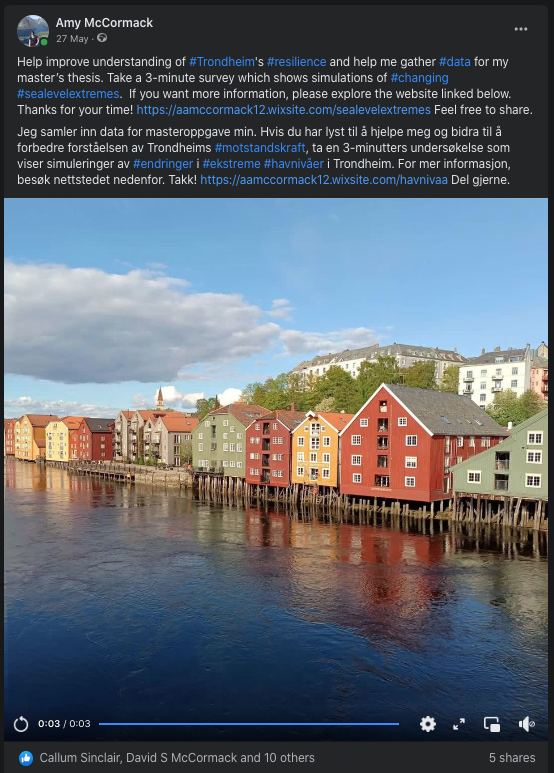
\includegraphics[width=0.9\textwidth]{fig_appendix/so_me.png}
    \caption{Social Media Post Used to Reach Subjects}{A short video playing a loop of the simulated water level extremes in Nidelva was utilised to optimise algorithms which prioritise video.}
    \label{fig:my_label}
\end{figure}


\begin{figure}
    \centering
    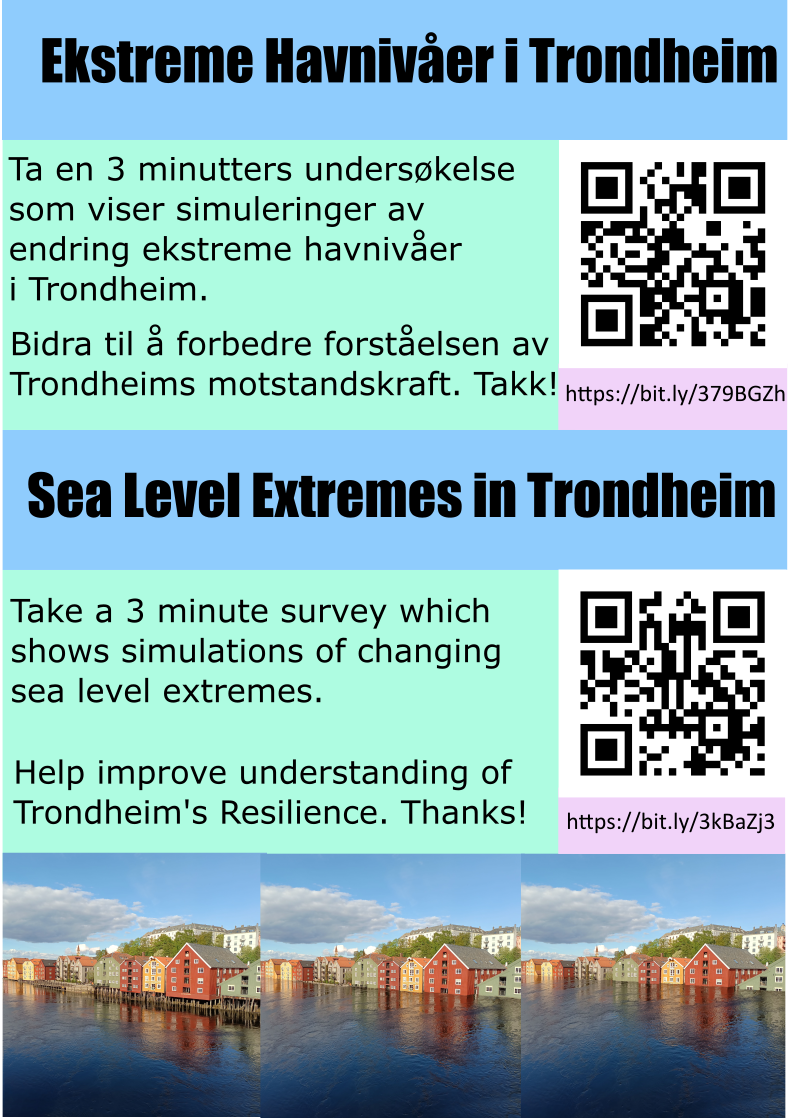
\includegraphics[width=0.9\textwidth]{fig_appendix/poster.png}
    \caption{This is the poster used to reach subjects}
    \label{fig:poster}
\end{figure}
    

